\documentclass[12pt]{article}

\usepackage{times}
\usepackage{textcomp}
\usepackage{listings}
\usepackage{fullpage}
\usepackage{color}
\usepackage{hyperref} 
\usepackage{pst-tree} 
\usepackage{verbatim} 
\usepackage{graphicx}
\usepackage{amsmath,amsfonts,amssymb,amsthm}

\graphicspath{ {./}}


\def\part#1{\item[\bf #1)]}
\renewcommand{\thesubsection}{Question \arabic{subsection}}

\author{Clement Tsang}

\begin{document}

\begin{center}
\Large\textbf{CS 241, Lecture 6 - Deterministic Finite Automata}
\end{center}

Note that from this point on, I'm using ``s'' to define ``\$'' when within code blocks.  

\section{Finite Languages and Membership}
\begin{itemize}
    \item Recall us defining languages and words.
    \item How can we efficiently determine membership for a finite language?  This is the easiest case.
    \item The naive way of doing it would be to check EVERY single word until we hit it or run through the entire list of words in the language.
    \item More efficiently, though, we could basically use a structure like a trie, where we determine if a word is in a language based on the previous character.
    \item For example:
\begin{lstlisting}[mathescape, numbers=none, breaklines=true]
if char[0] == 'b' {
    if char[1] == 'a' {
        if char[2] == 'g' {
            accept();
        }
        else if char[2] == 't' {
            accept();
        }
        else if no_more_chars(char*) reject();
    }
    else if char[2] == 'e' {
        if char[3] == 't' {
            accept();
        }
        else if no_more_chars(char*) reject();
    }
}
else reject();
\end{lstlisting}
    \item We can represent this pictorially: \\
        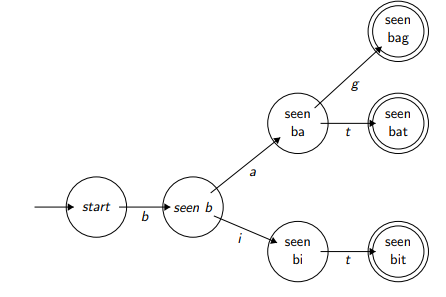
\includegraphics{pictorial_example.png}
    \item We place an arrow into the inital start state.
    \item Accepting states are two circles.
    \item Label your arrows from state to state.
    \item In CS 241, we do not need to include error states.  You'll need them for CS 360 though.  If your bubble does not have a valid arrow leaving it, we assume that this means it will go into an error state.
\end{itemize}


\section{Regular Languages}
\begin{itemize}
    \item A \textbf{regular language} over an alphabet $\sum$ consists of one of the following:
        \begin{enumerate}
            \item The empty language and the language consisting of the empty word are regular.
            \item All languages $\{s\}$ for all $s \in \sum$ are regular.
            \item The union, concatenation, or Kleene star of any two reg. lang. are also regular.
            \item Nothing else.
        \end{enumerate}
    \item Let $L, L_1, L_2$ be two reg. lang.  Then the following are regular languages:
        \begin{itemize}
            \item Union: $L_1 \bigcup L_2 = \{x : x \in L_1 \text{ or } x \in L_2\}$
            \item Concatenation: $L_1 \cdot L_2 = L_1L_2 = \{xy : x \in L_1, y \in L_2\}$
            \item Kleene star: $L* = \{\epsilon\} \bigcup \{xy : x \in L*, y \in L\} = \bigcup_{n=0}^{\infty} L^n$\\where $L^n = \begin{cases} \{\epsilon\} \text{ if } n = 0\\ LL^{n-1} \text{ otherwise}\end{cases}$
                \item Equivalently, $L*$ is the set of all strings consisting of 0 or more occurences of strings from $L$ concatenated together.
        \end{itemize}
    \item For example, suppose $L_1 =$ \{up, down\}, $L_2$ = \{hill, load\}, and $L = \{a, b\}$.  Then:
        \begin{itemize}
            \item $L_1 \bigcup L_2 = \{\text{up, down, hill, load}\}$
            \item $L_1L_2 = \{\text{uphill, upload, downhill, download}\}$
            \item $L* = \{\epsilon, a, b, aa, ab, ba, bb, aaa, aab, aba, \dots\}$
        \end{itemize}
    \item Another sample question: Let $\sum = \{a, b\}$. Explain why $L = \{ab^na : n \in \mathbb{N}\}$ is regular.
    \item \textbf{Solution:} Since $\{a\}$ is regular and $\{b\}*$ is also regular as $\{b\}$ is regular, then the concatenation of $\{a\} \cdot \{b\}* \cdot \{a\}$ is also regular.
    \item A regular expression is basically a regular language as well.  We just drop all the set notation.
        \begin{itemize}
            \item Union uses a pipe ($|$) now.
            \item Concationation is still $\cdot$ or just put them together.
            \item Kleene star stays the same.
            \item Order of operations: * $>$ $\cdot$ $>$ $|$.  
            \item For example, the previous example would translate to $ab*a$.
        \end{itemize}
\end{itemize}


\section{Deterministic Finite Automata}
\begin{itemize}
    \item We can use our earlier pictorial representation to represent a regular language IF we allow our picture to include loops!
    \item This is, of course, to support Kleene stars.  For example:\\
        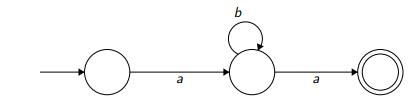
\includegraphics{loop.png}
    \item Or, if you're in CS 360: \\
        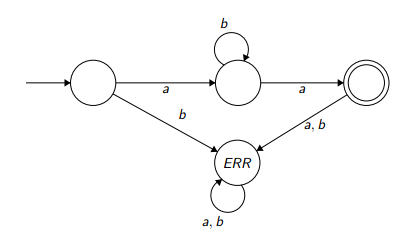
\includegraphics{loop_err.png}
    \item These machines are called \textbf{Deterministic Finite Automata (DFA):}
        \begin{itemize}
            \item A DFA is a 5-tuple ($\sum, Q, q_0, A, \delta$):
                \begin{itemize}
                    \item $\sum$ is a finite non-empty set (alphabet)
                    \item $Q$ is a finite non-empty set of states
                    \item $q_0 \in Q$ is a start state
                    \item $A \subseteq Q$ is a set of accepting states
                    \item $\delta : (Q \times \sum) \rightarrow Q$ is our transition function - given a state and a symbol of our alphabet, which state do we go to?  With no explicit arrows, this means, go to the error state.
                \end{itemize} 
        \end{itemize}
    \item For example, let's consider MIPS labels (Carmen forgot to add the image): \\
        -> [q0] -(a-z. A-Z)-> [q1](loops with (a-z, A-Z, 0-9)) -(:)-> [[q2]]
    \item Let's try another DFA example.  Write DFAs over $\sum = \{a, b\}$ that:
        \begin{enumerate}
            \item Accepts only words with an even number of $a$'s
            \item Accepts only words with an odd number of $a$'s and an even number of $b$'s
            \item Accepts only words where the parity of the number of $a$'s is equal to that of the number of $b$'s
        \end{enumerate}
        \newpage
    \item We'll do the third one:
        \begin{lstlisting}[mathescape, numbers=none, breaklines=true]
        -> [even a, even b] -a-> [odd a, even b] <-b-> [odd a, odd b]
                  ^
                  |
                  b                                         ^
                  V                                         |
            [even a, odd b] -b-> [even a, even b] -----<--a-|
        \end{lstlisting}
        <++>

\end{itemize}


\end{document}

